\documentclass[14pt, a4paper]{report}

%====================== PACKAGES ======================
\usepackage{extsizes}
\usepackage{tikz}
\usepackage[french]{babel}
\usepackage[utf8x]{inputenc}
\usepackage{hyperref}
\usepackage{multicol}
\usepackage[scale=0.8]{geometry}

\newenvironment{Figure}
  {\par\medskip\noindent\minipage{\linewidth}}
  {\endminipage\par\medskip}

\renewcommand{\baselinestretch}{1.25} 

\usepackage{caption}

\hypersetup{
    % bookmarks=true,         % show bookmarks bar?
    unicode=false,          % non-Latin characters in Acrobat’s bookmarks
    pdftoolbar=true,        % show Acrobat’s toolbar?
    pdfmenubar=true,        % show Acrobat’s menu?
    pdffitwindow=false,     % window fit to page when opened
    pdfstartview={FitH},    % fits the width of the page to the window
    pdftitle={Rapport},    % title
    pdfauthor={Loris},     % author
    pdfsubject={Prepro},   % subject of the document
    pdfcreator={},   % creator of the document
    pdfproducer={}, % producer of the document
    pdfkeywords={}, % list of keywords
    pdfnewwindow=true,      % links in new PDF window
    colorlinks=true,       % false: boxed links; true: colored links
    linkcolor=black,          % color of internal links (change box color with linkbordercolor)
    linkbordercolor=white,
    citecolor=green,        % color of links to bibliography
    filecolor=magenta,      % color of file links
    urlcolor=cyan           % color of external links
}

\usepackage[T1]{fontenc}

\author{Loïc \textsc{Castillo} -- Loris \textsc{Croce}}

\title{\rule{\textwidth}{1pt} \\ \Huge\textbf{Rapport de Pré-professionalisation : } \\ \emph{Enseignant-chercheur} \rule{\textwidth}{1pt}}

\begin{document}

\maketitle{}

\tableofcontents

\chapter{Présentation du métier}

  \section{Prérequis}

    \subsection{Formation}

    Afin d'être nommé à la place d'enseignement-chercheur dans une université publique, il est nécessaire d'obtenir un doctorat. Pour l'obtenir, le cursus classique est le suite d'études universitaire LMD (Licence / Master / Doctorat).
    Il est parfaitement possible d'obtenir le doctorat sans suivre ce cursus, bon nombre de chercheurs ont fait une commencer par une école préparatoire, puis ont continué sur une école d'ingénieur avant de revenir sur le cheminement classique.

    \begin{Figure}
      \centering
      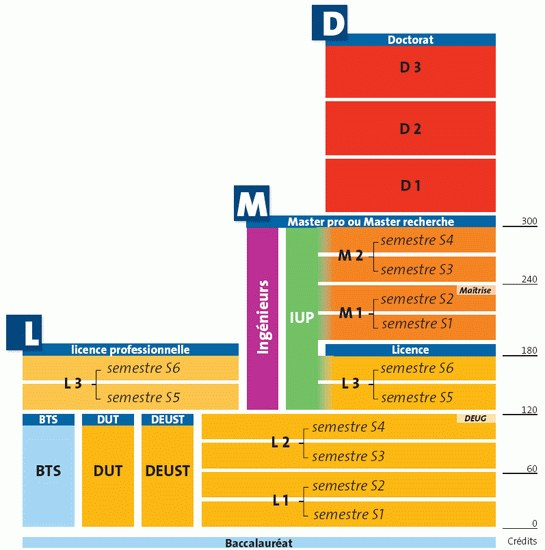
\includegraphics[width=6cm]{lmd.jpg}
      \captionof{figure}{schéma LMD}
    \end{Figure}

    \medskip

    Suite à cela, pour prétendre effectuer une candidature à un poste, il est nécessaire d'obtenir une accréditation de maitre de conférences qui est valable 4 ans.
		Outre l'université, on notera qu'il est également possible d'officier en entreprise dans les départements\ \emph{“Recherche \& Développement”}.

    \subsection{Compétences}

    Pour exercer ce métier il est préferable d’avoir une très bonne expression écrite et orale, une bonne connaissance de l’anglais ou encore de savoir travailler en groupe. Cependant ce ne sont pas les seuls critères, une veille constante des nouvelles technologies est nécessaire pour ne pas reproduire ce qui a déjà été fait ainsi qu’une bonne méthodologie de recherche pour un travail le plus efficace possible. 

    En effet, il faut procéder à une formation perpétuelle en se documentant sur le travail d’autres chercheurs, cela est d’autant plus vrai en informatique, où les progrès techniques sont extrêmement rapides.
    Savoir entretenir sa curiosité et son esprit critique sont des compétences importantes dans la profession.

  \section{Types de tâches à réaliser}

  Les tâches d'un enseignant-chercheur sont divisés en deux catégories. Nous allons en premier voir le travail à réaliser dans l'enseignement, puis nous verrons celui qui est lié au monde de la recherche.

    \subsection{Enseignement}

    Avant même d'obtenir le diplôme doctoral, un doctorant peut commencer à donner des cours, sous les instructions d'un directeur de thèse.
    Dans le domaine de l'informatique, les cours dispensés peuvent prendre la forme de Cours magistraux et de travaux dirigés ou pratiques. 

    L'activité d'enseignement comprend le cours donné en présentiel mais également la préparation du cours et la correction des travaux qui prend une part conséquente du temps d'enseignement.

    Dans certains cas un cours peut être dispensé par un intervenant (extérieur ou intérieur à la structure) qui n'est pas forcément enseignant-chercheur.

    \subsection{Recherche}

    L'activité de recherche est très différentes selon la personne et sa spécialité. Certains travailleront dans de gros projets internationaux, quand d'autres œuvreront en équipes réduites.
    Cette dernière comprend aussi un aspect gestion pour obtenir des financements et gérer des équipes selon le grade du chercheur.

    Cependant, la constante est l'activité de relecture et de publication qui reste indépendante de la discipline.

  \section{Lien avec les modules}

	Le cursus universitaire fournit un certain nombre de d'élements en lien avec le métier d'enseignant chercheur. D'une part sur les compétences pratiques qu'il fait mobiliser et d'une autre part sur les savoir théoriques qu'il inculque.

    \subsection{Compétences pratiques}

    % savoir travailler en autonomie -> Les TP, bosser chez soi. Publications -> rapport à rendre, bases théoriques indispensables -> algorithmique, théorie des graphes, mathématiques etc. -->

    Le travail exigé dans un cursus universitaire se rapproche de l'activité d'enseignement/recherche. En effet, les travaux à rendre nécessitent de savoir travailler en autonomie et/ou en équipe.
    Le mode d'enseignement favorise l'approfondissement de ce qui est enseigné en cours et force à développer son esprit critique et sa faculté à rechercher des informations.

    On pourra aussi faire le lien entre les travaux à rendre à l'écrit ou à présenter à l'oral qui font écho à ce qui est réalisé dans le quotiden de la recherche.

    \subsection{Compétences théoriques}

    D'un point de vue plus scolaire, l'ensemble des modules enseignés font écho savoir nécessaire pour un chercheur en informatique.

    Le cursus de licence fournit une base dans l'ensemble des champs étudiés en informatique, comme les bases de données, le génie logiciel, l'algorithmique, la théorie des graphes\dots\ qui sont indispensables pour une carrière dans la recherche et l'enseignement en informatique.

    En master une spécialisation dans un domaine s'effectue et peut éventuellement permettre d'orienter un sujet de thèse.

\chapter{Outils}

  \section{Littérature scientifique}

  L'outil primordial quand on effectue une activité de recherche est de s'appuyer sur la littérature scientifique ses travaux.

	  \subsection{Le libre accès}

	  Dans une optique de diffusion de la connaissance dans l'intérêt général, certaines revues scientifiques sont en libre accès et suivent le modèle d'\emph{auteur-payeur}.
	  On pourra citer : \emph{INFOCOMP Journal of Computer Science, JOT: Journal of Object Technology, Journal of Artificial Intelligence Research, Journal of Machine Learning, Research, Logical Methods in Computer Science, Theory of Computing}

	  Il existe aussi en complément une plate-forme, HAL, \emph{Hyper Articles en Lignes} qui met à disposition un ensemble de publications scientifiques et permet à tous chercheur d'y déposer son travail. Cependant ces publications ne sont pas  \emph{évaluées} par un comité scientifique.

	  \subsection{Les revues payantes}

	  Une grande partie de des publications scientifiques sont publiés dans des revues payantes, elles sont généralement achetées par les laboratoires et les chercheurs qui publient dedans ne sont pas rémunérés par l'éditeur de la revue.
	  Il y a cependant un grand intérêt pour les chercheurs à publier dans ces revues, en effet ceux-ci sont évalués notamment sur la quantité de leurs publications et de la \emph{réputation} de la revue dans laquelle est ils publient.

  \section{Autre}

  D'autres outils sont généralement utilisés dans le milieu de l'enseignement et la recherche. Pour la publication d'articles le logiciel \LaTeX est souvent utilisé car il facilite la mise en forme de rapport, articles et des livres ainsi que l'écriture de formules mathématiques.

  On pourra aussi citer des logiciels utilisés en recherche tels que :
  \begin{itemize}
  	\item \textbf{R}, un langage destiné au traitement de données.
  	\item \textbf{Matlab}, un logiciel destiné au calcul numérique. Et ses alternatives libres GNU Octave ou SageMath.
  	\item \textbf{Maple}, un logiciel destiné au calcul formel.
  \end{itemize}

\chapter{Journée des métiers}

Lors de cette jounée des métiers, des professionnels sont venus nous présenter leur travail et le fonctionnement de leurs entreprises, puis 4 étudiants sont venus partager leur expérience dans le monde dans le monde de la Recherche.

\section{Matinée}

Les 3 premières entreprises furent STERIA-SOPRA, CGI (Conseil, Intégration et Outsourcing) et ATOS, toutes des ESN, \emph{Entreprises de Services Numériques}. Celles-ci ont présenté les méthodes de travail de leurs entreprises, elles ont insisté sur le fait que le travail devait être effectué en équipe, la pratique de l'anglais orale étant un point important car les projets peuvent être internationaux, en raison de collaboration avec des sous-traitants étrangers. Par ailleurs, ces entreprises ont bien appuyé sur le fait que un développeur ne passerait pas tout son temps à coder, mais que les phases d'analyse et de gestion de projet en amont étaient aussi très importantes. Ils mirent également l'accent sur leur motivation à embaucher des alternants et des stagiaires dans notre corps de métier.

Nous avons pu aussi entendre le récit de développeurs de ces entreprises qui étaient pour la plupart des anciens étudiants, leur discours étaient unanime, diversité de projet, équipe soudée, ambiance satisfaisante, le tout sous le regard de leurs managers.

\section{Après-midi}

\subsection{Conférences}

\subsubsection{Julien Ponge} Maître de conférences à l'INSA Lyon tout en étant développeur au sein de l'entreprise Red Hat. M. \textsc{Ponge} a obtenu une licence et un master à l'Université Blaise Pascal, puis un doctorat à l'Université de Grenoble. Après avoir pratiqué la fonction d'enseignant-chercheur, il s'est rapproché du domaine privé afin d'obtenir une nouvelle expérience, tout en continuant d'enseigner à l'INSA. À Red Hat il travaille sur Vert.x, un framework Java basé sur les évènements, permettant d'obtenir une augmentation des performances.

\subsubsection{Valerian Callens} Auditeur des Systèmes d'Informations à la Société Générale nous a présenté son parcours et son métier depuis son lieu de travail en Roumanie. Avant de commencer sa carrière, M. Callens avait fait un V.I.E. (Volontariat International en Entreprise) de deux ans au sein de la Société Générale, cela lui a permit de découvrir la Roumanie, acquérir de l'expérience et vérifier que ce métier lui correspondait bien. Son métier consiste à observer les risques et faire des contrôles, afin de protéger des systèmes d'informations dont il a la charge.

\subsubsection{Frederic Andrès} Maître de conférences au NII, \emph{National Institute of Informatics} de Tokyo, nous a presenté son activité dans le département de contenus numériques et les sciences des médias. Il nous a aussi expliqué les démarches nécessaires pour effectuer un stage au NII.


\subsection{Doctorants}

Après ce cycle de conférences, 2 doctorants sont venus présenter leur projet de recherche.

L'une d'eux, après avoir fait une école Polytechnique suivi d'un Master, effectue sa thèse au sein de Michelin, en tant que salariée, dans le cadre d'une thèse CIFR. Elle travaille sur l'analyse de données télémétriques afin de pouvoir anticiper l'usure des pneus. Étant donné que cette chercheuse est salariée de Michelin, le résultat de ses travaux doivent permettre à Michelin de dégager une valeur ajoutée.

Un autre étudiant travaille sur l'analyse du comportement des vaches, lors de leur repos, ou de leur période d'alimentation, afin de détecter à l'avance si elles vont être malades. Sa thèse est effectuée en partenariat avec l'INRA qui participe à son financement.


\end{document}